%!TEX root = ../dokumentation.tex

\chapter{Grundlagen / Methodischer Ansatz}


\section{SAP TwoGo}

In zahlreichen Gesellschaftsbereichen spielen Nachhaltigkeit und Umweltschutz aktuell eine bedeutende Rolle. Auch Unternehmen haben dies erkannt und möchten verstärkt umweltschonend handeln. Eine ganz konkrete Thematik ist hierbei unter anderem der Arbeitsweg der Mitarbeiter, da ein Großteil oft weite Strecken alleine zurücklegt, um zur Arbeit zu gelangen.\footnote{Vgl. \cite{SAP}} Laut Schindler pendeln in Deutschland jeden Tag 32 Millionen Arbeitnehmer zur Arbeit. Daraus ergeben sich Kosten in Höhe von 700 Millionen Euro pro Tag.\footnote{\cite{silicon}} Außerdem geht damit einher, dass das Staurisiko steigt und die Kraftstoffkosten für den Einzelnen sehr hoch sind. \\
An dieser Stelle setzt TwoGo by SAP an.\footnote{Vgl. \cite{SAP}} TwoGo stellt den Mitarbeitern eine Plattform zur Bildung von Fahrgemeinschaften zur Verfügung. Dadurch lassen sich zum einen die schädlichen Treibhausemissionen senken und zum anderen können die Treibstoffkosten reduziert werden. Diese Vorteile sind sowohl für den Arbeitnehmer positiv einzustufen, da sein Geldbeutel geschont wird, als auch für den Arbeitgeber, da seine Umweltbilanz verbessert wird, die Kosten für die Wartung seiner Firmenwagenflotte verringert werden und der Wiederverkaufswert der Firmenwagen steigt.\\
Aber nicht nur aus wirtschaftlicher Sicht bringt TwoGo Vorteile, auch der Mensch profitiert, da er bei gemeinsamen Fahrten zur Arbeit neue Kollegen kennenlernen kann. Zudem kann auch die Beziehung zwischen dem Unternehmen und dem einzelnen Mitarbeiter unter anderem in Form von zusätzlichen Leistungen für TwoGo-Nutzer gestärkt werden. Diese Leistungen könnten zum Beispiel besonders gut gelegene Parkplätze sein, die nur von Fahrgemeinschaften genutzt werden dürfen. Schon diese Argumente zeigen deutlich, welche Vorteile eine solche Plattform mit sich bringen kann.\\
Damit diese Plattform optimal eingesetzt werden kann, muss eine ortsunabhängige und unternehmensübergreifende Nutzung, am besten im Form einer Cloud, gewährleistet werden. Um diese zwei wichtigen Punkte sicherzustellen, wird TwoGo in SAP Rechenzentren gehostet. Dies gewährleistet außerdem ein hohes Maß an Sicherheit und eine durchgehende Erreichbarkeit von TwoGo. Damit auch der Endanwender von der Cloud profitiert und auch jederzeit auf TwoGo zugreifen kann, gibt es insgesamt zwei Wege, TwoGo zu nutzen: entweder über einen PC/Laptop oder über ein Smartphone. Am PC lässt sich auf TwoGo über den Internet Browser oder Microsoft Outlook zugreifen und am Smartphone über die mobile Internetseite oder die native App. Somit ist der Zugriff immer gewährleistet und der Anwender kann zu jeder Zeit eine Mitfahrgelegenheit suchen oder anlegen.




%\\cite[vgl. S. 10f.]{PLM_beherrschen}

%\begin{figure}[H]
%    \centering
%    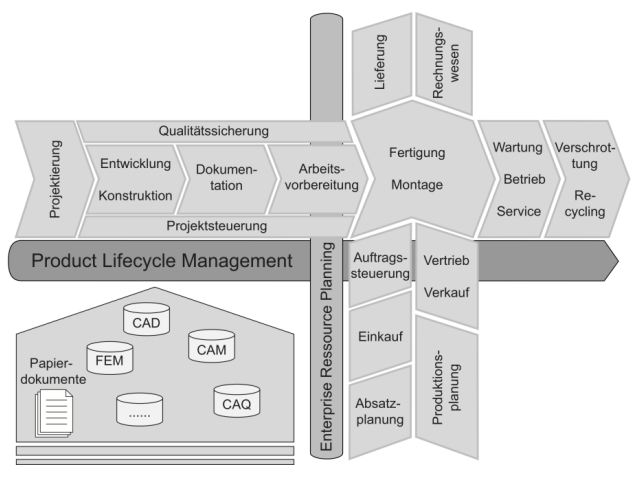
\includegraphics[width=0.7\textwidth]{PLM_beherrschenSeite10.JPG}
%    \caption{Konzept des \acl{PLM}}  \cite[Seite 10]{PLM_beherrschen}
%  \label{img:konzeptPLM}
%  
%\end{figure}

\section{Entwicklungslandschaft}
Um TwoGo regelmäßig und relativ zügig mit neuen Funktionen und Bugfixes zu versorgen\footnote{Vgl. \cite{wiki}}, wird bei der Entwicklung Scrum genutzt. Dies ermöglicht es, Softwareentwicklung nach den Grundsätzen der agilen Softwareentwicklung durchzuführen. Zur Unterstützung des Scrum Prozesses wird als Project Management Tool \textit{Trac} eingesetzt. Es ermöglicht das zentrale Speichern von Dokumentation, Stories, Fehlern und Aufgaben. \\
Die Entwickler programmieren das TwoGo Backend mithilfe der Entwicklungsumgebung \textit{Eclipse} und nutzen Java als Programmiersprache. Für die Oberfläche wird JavaScript und HTML eingesetzt. Zur Datenhaltung wird eine \textit{SAP MaxDB} Datenbank genutzt. Damit die einzelnen Veränderungen in den Quelldateien jederzeit nachverfolgt und gegebenenfalls zurückgenommen werden können, wird ein \acl{VCS} genutzt. Momentan werden hierfür \textit{Perforce} und \textit{git} eingesetzt. Aus den Quelldateien werden mithilfe von \textit{Maven} Binärdateien erzeugt, welche danach in einer \acs{WAR}-Datei\footnote{Vgl. \cite[Seite 329]{danny_java_????}} gepackt  und auf einem zentralen Server, dem sogenannten \textit{Nexus}, abgelegt werden.\\
Um kontinuierliches Kompilieren von Quelldateien, automatisiertes Testen und Ausrollen von Binärdaten zu ermöglichen, wird \textit{Jenkins} als \acl{CI} System verwendet. Dabei nutzt \textit{Jenkins} die bereits erwähnten Komponenten \textit{\acs{VCS}, Maven} und den \textit{Nexus}. Das Zusammenwirken dieser wird mithilfe Abbildung \ref{fig:Server} dargestellt. Die Funktion der Komponenten und deren Zweck werden ausführlich in Kapitel 3 erläutert.%\textit{Jenkins} ermöglicht außerdem auch das automatische Ausrollen der Binärdateien auf Entwicklungsserver.

\section{Aktueller Deploymentprozess}
In der Entwicklung von SAP TwoGo gibt es drei Landschaften (Abbildung \ref{fig:Server}): eine \textit{Dev-Landschaft} (Entwicklungslandschaft), eine \textit{Patch-Landschaft} (Testlandschaft) und eine \textit{Cons-Landschaft} (Produktivlandschaft).\footnote{Vgl. \cite{wiki}} Diese Landschaften haben jeweils drei Server: einen Datenbankserver und zwei Backend-Server (Matcher, Matchfinder). Durch die Verwendung mehrerer Landschaften wird gewährleistet, dass Entwickler, Tester und Anwender ein eigenständiges System haben.
\begin{figure}[H]
\centering
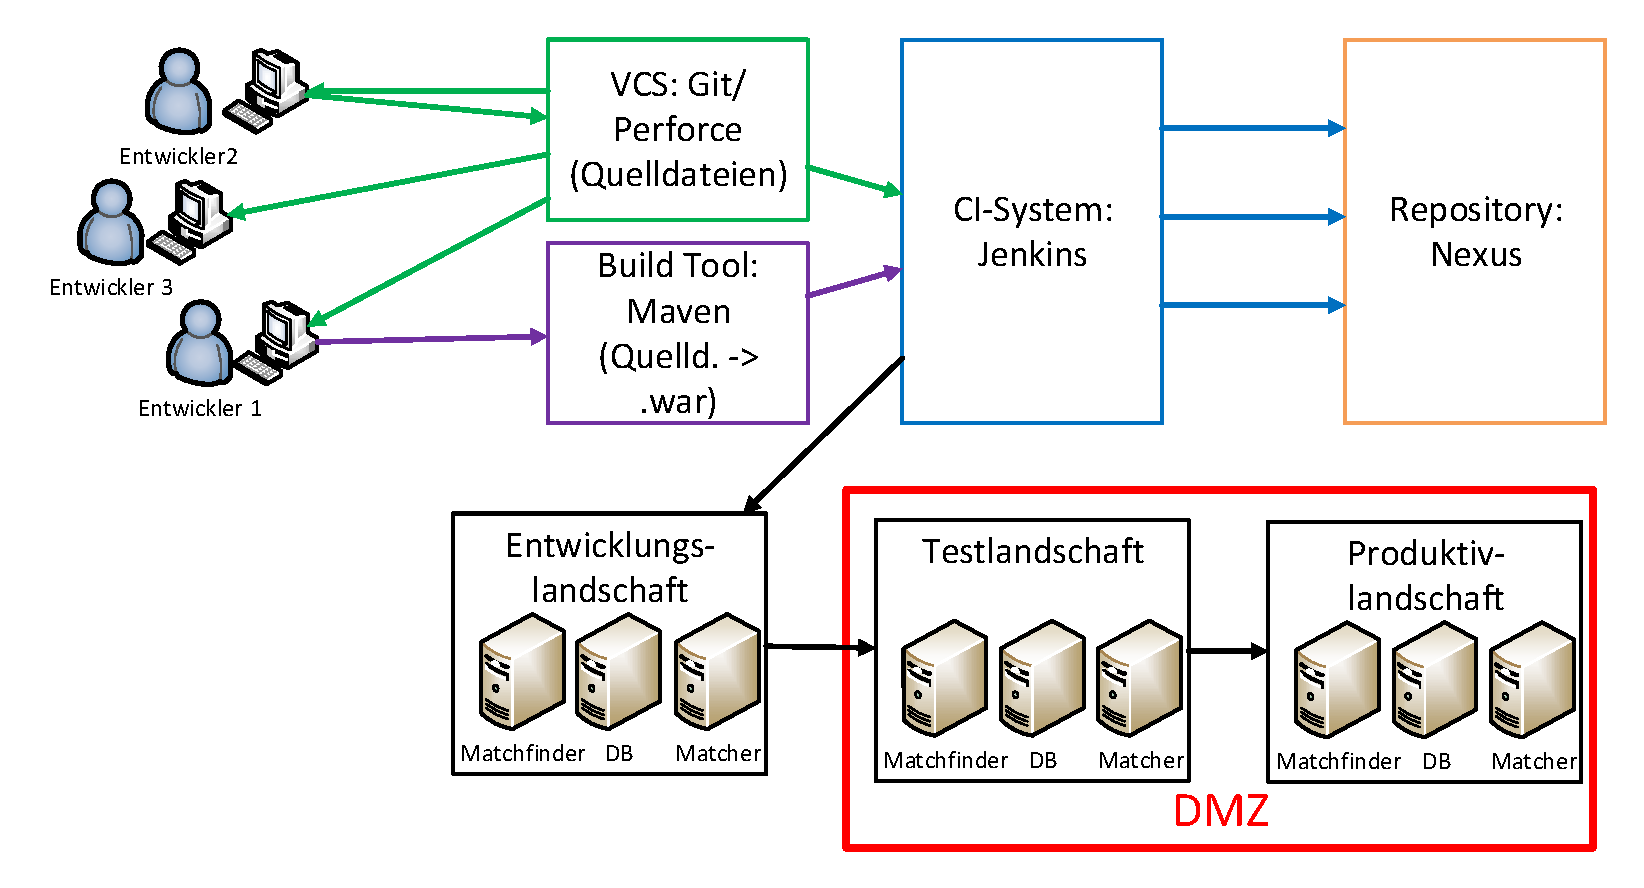
\includegraphics[width=1\linewidth]{../images/Server_Struktur2.pdf}
\vspace{-30pt}
\caption{TwoGo Server}
\label{fig:Server}
\vspace{-10pt}
\end{figure}
Soll nun eine bestimmte Version von TwoGo von der Entwicklungslandschaft auf die Produktivlandschaft oder Testlandschaft transportiert werden, spricht man von Deployment. Diesen Deploymentprozss kann man bei SAP TwoGo aus zwei Perspektiven betrachten, aus der technischen sowie der organisatorischen Sicht.\\
Organisatorisch ist der Deploymentprozess stark an die unternehmensinterne Struktur und an interne Regelungen von SAP gebunden. Zunächst wird ein \textit{Quality Gate} Meeting durchgeführt. Dabei wir anhand von festgelegten Qualitätskriterien beschlossen, ob ein neuer Release stattfindet und wenn ja, welche Features ausgerollt werden sollen. Daraufhin müssen weitere Abteilungen durchlaufen werden. Eine dieser Abteilungen prüft beispielsweise die verwendeten open-source Bibliotheken, während eine andere den gesamten Quellcode auf potentielle Sicherheitslücken überprüft. Dies führt dazu, dass der Deploymentprozess sehr zeitaufwendig ist, wodurch ein neuer Release momentan nur alle drei Wochen möglich ist.\\
Auf der technischen Seite müssen zwei unterschiedliche Fälle unterschieden werden. Möchte der Entwickler etwas auf die Entwicklungslandschaft ausbringen, so kann er dies mithilfe von Jenkins (siehe Kapitel 2.3 und 3.2) über ein Deployment Skript vollautomatisch ablaufen lassen.\\
Bei den anderen beiden Landschaften (Test und Produktiv) ist dies komplizierter. Bereits das Zugreifen auf die Server ist nicht einfach, da sich diese innerhalb einer Sicherheitszone, der sogenannten \acs{DMZ} (demilitarisierte Zone), befinden. Zugriff auf diese Landschaften ist nur über \acs{WTS} und unter Einhaltung strenger Sicherheitsrichtlinien manuell möglich. Hat man diese Barriere passiert, müssen die frisch kompilierten Binärdateien mithilfe eines Deployment Skriptes deployed werden. Dabei kommt es allerdings manchmal zu Komplikationen, wenn Dateien in einer falschen Version vorliegen, woraufhin diese manuell geändert und kopiert werden müssen. 
Da die Binärdateien bei jedem Deployment und für jede Landschaft neu kompiliert werden, entstehen überflüssige Redundanzen. Ein weiteres Problem sind die verwendeten open-source Bibliotheken, welche zentral auf dem Nexus gespeichert werden, weil diese gelegentlich in einer falschen Version vorliegen. Dadurch können Folgefehler beim Kompilieren entstehen. All diese Probleme führen dazu, dass sich das Deployment auch aus technischer Sicht  in die Länge zieht.\\
Insgesamt verdeutlichen diese beiden Perspektiven die Zeitbeanspruchung und die Fehleranfälligkeit, welche ein schnelleres Deployment verhindern. %\footnote{Vgl. \cite{wiki}}



\section{Unix}
Die Server in der TwoGo Entwicklungslandschaft nutzen sowohl Unix-basierte Betriebssysteme als auch Microsoft Windows. Betrachtet man zudem die heutige Verteilung von Betriebssystemen\footnote{\cite{Umfrage_OS}}, so erkennt man, dass nur diese zwei Arten von Betriebssystemen auf dem Markt verbreitet sind.\\
Die bekanntesten Vertreter von Unix-Betriebssystemen sind Mac OS X von Apple, Linux, FreeBSD sowie Android von Google. Schon an diesen vier Beispielen lässt sich das Einsatzspektrum von Unix-Betriebssystemen gut abschätzen, welches beim Server beginnt und beim Smartphone endet. Ihre Gemeinsamkeit besteht darin, dass alle die grundlegenden Konzepte von Unix nutzen. Zu den wichtigen Konzepten von Unix gehören zum einen die Schnittstellen und zum anderen das Dateisystem. \\
Unix lässt sich in fünf Schichten unterteilen\footnote{Vgl. \cite[Seite 11ff]{systemprogrammierung_2011}}, wodurch ein  modularer Aufbau gewährleistet wird, der es auch ermöglicht, einzelne Schichten auszutauschen. Abbildung \ref{img:Schichtenmodell} zeigt diese Schichten. Sie folgen einem logischen Aufbau, der  mit der Hardware beginnt und  mit dem Benutzer endet. Elementare Funktionen, wie die Prozessverwaltung, sind vom Benutzer entkoppelt. Auf die einzelnen Funktionen der Schichten kann über Schnittstellen, wie beispielsweise die Systemaufrufschnittstelle, zugegriffen werden. Somit fungieren die Schnittstellen als Verbindung zwischen den einzelnen Schichten.

\begin{figure}[H]
    \centering
    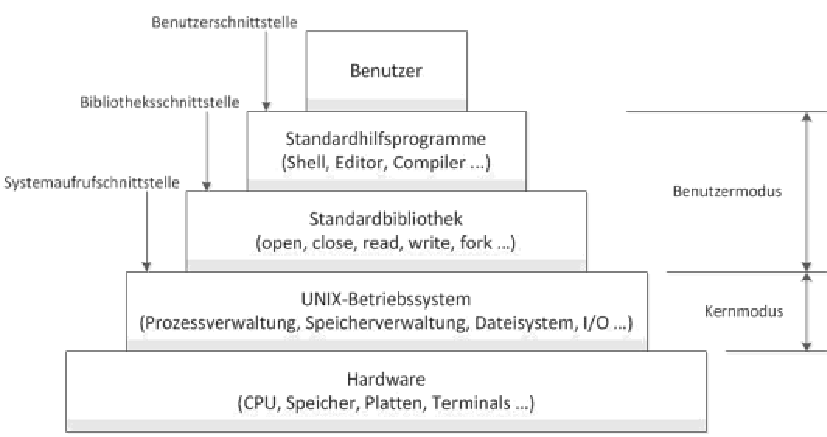
\includegraphics[width=0.75\textwidth]{Schichtenmodell.pdf}
    \vspace{-10pt}
    \caption{Unix Schichtenmodell} \cite[Seite 12]{systemprogrammierung_2011}
    \vspace{-20pt}
  \label{img:Schichtenmodell}
\end{figure}

Die zweite Besonderheit von Unix-Betriebssystemen liegt, wie oben genannt, in der Dateistruktur.\footnote{Vgl. \cite[Seite 7ff]{burtch_linux_2004}}  Diese ist baumartig aufgebaut und gruppiert Dateien nach ihrer Art und Zugehörigkeit. Hierdurch ist die Struktur unabhängig von der Hardware, das heißt, es gibt keine Laufwerke wie man es von Windows kennt. Die grundlegende Dateistruktur ist in der folgenden Grafik \ref{img:Dateistruktur} dargestellt:

\begin{figure}[H]
    \centering
    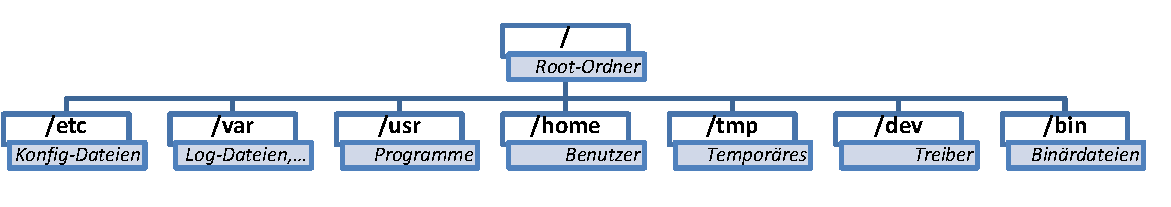
\includegraphics[width=1.1 \textwidth]{Dateistruktur.pdf}
    \vspace{-20pt}
    \caption{Unix Dateistruktur}
    \vspace{-10pt}
  \label{img:Dateistruktur}
\end{figure}



\section{Shell-Programmierung mit Bash}
Die meisten Betriebssysteme nutzen grafische Oberflächen, um dem Anwender ein einfaches Arbeiten zu ermöglichen, es gibt jedoch Situationen, in denen grafische Oberflächen ineffektiv werden. Wenn man zum Beispiel den Dateinamen aller Dateien in einem Verzeichnis mit einer fortlaufender Nummer versehen will, ist dies über die grafische Oberfläche sehr umständlich. In solchen Situationen ist es effizienter, die Kommandozeile zu benutzen. Mit dieser lassen sich bestimmte Systembefehle aufrufen. Im eben genannten Beispiel benennt der Befehl \textit{rename} Dateien oder Verzeichnisse um.\\ Aber auch die Kommandozeile hat den Nachteil, dass der Anwender immer den Befehl manuell eingeben muss. Bei einmaligen Tätigkeiten, wie dem Umbenennen von Dateien stellt dies noch kein Problem dar. Möchte man jedoch zum Beispiel bei Systemstart automatisch die neuesten Dateien von einem Server herunterladen, ist selbst die Kommandozeile nicht mehr effektiv. Nun hat man zwei Möglichkeiten. Entweder man schreibt in einer beliebigen Programmiersprache ein entsprechendes Programm oder man \textit{automatisiert} die Kommandozeile. Letzteres nennt man \textit{scripting} oder \textit{Shell-Programmierung}. Man erstellt dabei ein sogenanntes \textit{Shell Script}. Dies ist im Wesentlichen eine einfache Textdatei, welche mit Kommandozeilen-Befehlen gefüllt ist.\\
Unter Unix gibt es verschiedene Shell-Arten\footnote{Vgl. \cite[Seite 4]{burtch_linux_2004}}, die sich hauptsächlich in ihrer Syntax und der Befehlsvielfalt unterscheiden. Trotz einer Vielzahl von Shell-Arten sind viele von ihnen sehr ähnlich. Die wohl am meisten genutzte Shell ist \acs{Bash}. Diese funktioniert sowohl unter Linux als auch unter OS X und ist für jeden frei zugänglich (open-source). In der Fachliteratur wird \acs{Bash} oft auch als \textit{Quasi-Standard} bezeichnet.\\
Um ein Shell-Skript zu schreiben\footnote{Vgl. \cite[Seite 23]{shell-programmierung}}, benötigt man nur einen Texteditor, welcher in der Regel bei jedem Betriebssystem bereits vorinstalliert ist. Damit das System die Datei richtig interpretieren kann, muss in der ersten Zeile des Skriptes lediglich das  \textit{She-Bang (\#!)} in Verbindung mit der verwendeten Shell-Art stehen. Bei Bash sieht dies folgendermaßen aus:\textit{ \#!/bin/bash }. Damit sind die Grundlagen für ein Shell-Skript gegeben und man kann somit auch die weiteren Vorteile von Shell-Skripten nutzen. So bietet \acs{Bash} die Möglichkeit, Variablen, Bedingungen, Schleifen und Unterprogramme zu verwenden.\\
Es folgt nun ein Skript, das automatisch Daten von einem Server herunterlädt und in den entsprechenden Ordner verschiebt. An diesem Beispiel kann man gut erkennen, wie ein \acs{Bash}-Skript aufgebaut ist. In diesem Beispiel sind Befehle fett markiert und Kommentare werden mit einem \textit{\#} eingeleitet.
\begin{lstlisting}
#!/bin/bash
#Laedt die neusten *.war Dateien herunter
#########################################
#Variablen deklarieren
declare  TEMP_LOC=/tmp/warfiles		#Tmp Verzeichnis
declare  TGT_LOC=/home/deploy		#Zielort
#Tmp Ordner erstellen
mkdir -p $TEMP_LOC
cd $TEMP_LOC						# Verzeichnis wechseln
#Download
wget -q "http://server:8010/attachment/kraftwerk.war" 
wget -q "http://server:0380/attachment/web.war" 

mv -u kraftwerk.war $TGT_LOC 		#Datei 1 verschieben
mv -u web.war $TGT_LOC			    #Datei 2 verschieben
rm -fr $TEMP_LOC		            #Tmp Verzeichnis loeschen
kill 0		                        #Skript beenden
\end{lstlisting}

